% ============================================================
% Question Bank: ch04-04 Factoring Expressions
% Topic Title: Factoring Expressions
% CCSS: 7.EE.A.1
% Questions: 30 (18 MC + 7 SA + 5 Graphical)
% ============================================================

% --- Multiple Choice Questions (18) ---

\begin{practiceQuestion}{4-4-q01}{mc}
\begin{questionText}
What is the greatest common factor (GCF) of $12$ and $18$?
\end{questionText}
\choiceA{$2$}
\choiceB{$3$}
\choiceC{$6$}
\choiceD{$9$}
\correctAnswer{C}
\explanation{Factors of $12$: $1, 2, 3, 4, 6, 12$. Factors of $18$: $1, 2, 3, 6, 9, 18$. The greatest common factor is $6$.}
\end{practiceQuestion}

\begin{practiceQuestion}{4-4-q02}{mc}
\begin{questionText}
Factor $6x + 12$.
\end{questionText}
\choiceA{$2(3x + 6)$}
\choiceB{$6(x + 2)$}
\choiceC{$3(2x + 4)$}
\choiceD{$6(x + 12)$}
\correctAnswer{B}
\explanation{GCF of $6x$ and $12$ is $6$. Factor: $6x \div 6 = x$ and $12 \div 6 = 2$. Result: $6(x + 2)$.}
\end{practiceQuestion}

\begin{practiceQuestion}{4-4-q03}{mc}
\begin{questionText}
Factor $15a - 10$.
\end{questionText}
\choiceA{$5(3a - 2)$}
\choiceB{$5(3a + 2)$}
\choiceC{$3(5a - 10)$}
\choiceD{$10(a - 1)$}
\correctAnswer{A}
\explanation{GCF of $15$ and $10$ is $5$. Factor: $15a \div 5 = 3a$ and $-10 \div 5 = -2$. Result: $5(3a - 2)$.}
\end{practiceQuestion}

\begin{practiceQuestion}{4-4-q04}{mc}
\begin{questionText}
Which is the completely factored form of $8m + 20$?
\end{questionText}
\choiceA{$2(4m + 10)$}
\choiceB{$4(2m + 5)$}
\choiceC{$8(m + 20)$}
\choiceD{$4(2m + 20)$}
\correctAnswer{B}
\explanation{GCF of $8$ and $20$ is $4$. Factor: $8m \div 4 = 2m$ and $20 \div 4 = 5$. Result: $4(2m + 5)$. Choice A uses $2$, which is not the GCF.}
\end{practiceQuestion}

\begin{practiceQuestion}{4-4-q05}{mc}
\begin{questionText}
Factor $14x + 21y$.
\end{questionText}
\choiceA{$7(2x + 3y)$}
\choiceB{$7(2x + 21y)$}
\choiceC{$14(x + y)$}
\choiceD{$3(4x + 7y)$}
\correctAnswer{A}
\explanation{GCF of $14$ and $21$ is $7$. Factor: $14x \div 7 = 2x$ and $21y \div 7 = 3y$. Result: $7(2x + 3y)$.}
\end{practiceQuestion}

\begin{practiceQuestion}{4-4-q06}{mc}
\begin{questionText}
Factor $-9x - 6$.
\end{questionText}
\choiceA{$-3(3x - 2)$}
\choiceB{$-3(3x + 2)$}
\choiceC{$3(-3x - 2)$}
\choiceD{$-9(x + 6)$}
\correctAnswer{B}
\explanation{GCF is $3$. Factor out $-3$: $-9x \div (-3) = 3x$ and $-6 \div (-3) = 2$. Result: $-3(3x + 2)$. Check: $-3(3x + 2) = -9x - 6$ \checkmark.}
\end{practiceQuestion}

\begin{practiceQuestion}{4-4-q07}{mc}
\begin{questionText}
Which expression cannot be factored (has GCF of $1$)?
\end{questionText}
\choiceA{$6x + 9$}
\choiceB{$4a - 10$}
\choiceC{$5n + 7$}
\choiceD{$12y + 8$}
\correctAnswer{C}
\explanation{GCF of $5$ and $7$ is $1$, so $5n + 7$ cannot be factored further. All other expressions have a GCF greater than $1$.}
\end{practiceQuestion}

\begin{practiceQuestion}{4-4-q08}{mc}
\begin{questionText}
Factor $24x - 16$.
\end{questionText}
\choiceA{$4(6x - 4)$}
\choiceB{$8(3x - 2)$}
\choiceC{$2(12x - 8)$}
\choiceD{$6(4x - 2)$}
\correctAnswer{B}
\explanation{GCF of $24$ and $16$ is $8$. Factor: $24x \div 8 = 3x$ and $-16 \div 8 = -2$. Result: $8(3x - 2)$.}
\end{practiceQuestion}

\begin{practiceQuestion}{4-4-q09}{mc}
\begin{questionText}
A student factors $10x + 25$ as $5(2x + 25)$. What error did the student make?
\end{questionText}
\choiceA{Used the wrong GCF}
\choiceB{Divided only the first term by the GCF}
\choiceC{Factored out a negative instead of a positive}
\choiceD{Added the terms instead of dividing}
\correctAnswer{B}
\explanation{The student divided $10x$ by $5$ to get $2x$, but did not divide $25$ by $5$. The correct factoring is $5(2x + 5)$.}
\end{practiceQuestion}

\begin{practiceQuestion}{4-4-q10}{mc}
\begin{questionText}
Factor $18a + 12b + 6$.
\end{questionText}
\choiceA{$6(3a + 2b + 1)$}
\choiceB{$3(6a + 4b + 2)$}
\choiceC{$2(9a + 6b + 3)$}
\choiceD{$6(3a + 2b + 6)$}
\correctAnswer{A}
\explanation{GCF of $18$, $12$, and $6$ is $6$. Divide each: $18a \div 6 = 3a$, $12b \div 6 = 2b$, $6 \div 6 = 1$. Result: $6(3a + 2b + 1)$.}
\end{practiceQuestion}

\begin{practiceQuestion}{4-4-q11}{mc}
\begin{questionText}
Factor $-12y + 8$.
\end{questionText}
\choiceA{$4(-3y + 2)$}
\choiceB{$-4(3y + 2)$}
\choiceC{$-4(3y - 2)$}
\choiceD{Both A and C}
\correctAnswer{D}
\explanation{$4(-3y + 2) = -12y + 8$ \checkmark. Also $-4(3y - 2) = -12y + 8$ \checkmark. Both are valid factored forms.}
\end{practiceQuestion}

\begin{practiceQuestion}{4-4-q12}{mc}
\begin{questionText}
Factor $20n - 30$.
\end{questionText}
\choiceA{$5(4n - 6)$}
\choiceB{$10(2n - 3)$}
\choiceC{$2(10n - 15)$}
\choiceD{$20(n - 30)$}
\correctAnswer{B}
\explanation{GCF of $20$ and $30$ is $10$. Factor: $20n \div 10 = 2n$ and $-30 \div 10 = -3$. Result: $10(2n - 3)$.}
\end{practiceQuestion}

\begin{practiceQuestion}{4-4-q13}{mc}
\begin{questionText}
Which expression is equivalent to $3(4x - 7)$?
\end{questionText}
\choiceA{$12x - 7$}
\choiceB{$12x + 21$}
\choiceC{$12x - 21$}
\choiceD{$7x - 21$}
\correctAnswer{C}
\explanation{Expand to verify: $3 \times 4x = 12x$ and $3 \times (-7) = -21$. So $3(4x - 7) = 12x - 21$.}
\end{practiceQuestion}

\begin{practiceQuestion}{4-4-q14}{mc}
\begin{questionText}
Factor $16x + 24y - 8$.
\end{questionText}
\choiceA{$4(4x + 6y - 2)$}
\choiceB{$8(2x + 3y - 1)$}
\choiceC{$2(8x + 12y - 4)$}
\choiceD{$8(2x + 3y + 1)$}
\correctAnswer{B}
\explanation{GCF of $16$, $24$, and $8$ is $8$. Divide each: $16x \div 8 = 2x$, $24y \div 8 = 3y$, $-8 \div 8 = -1$. Result: $8(2x + 3y - 1)$.}
\end{practiceQuestion}

\begin{practiceQuestion}{4-4-q15}{mc}
\begin{questionText}
Factor $-15a + 25$.
\end{questionText}
\choiceA{$5(-3a + 5)$}
\choiceB{$-5(3a + 5)$}
\choiceC{$-5(3a - 5)$}
\choiceD{Both A and C}
\correctAnswer{D}
\explanation{$5(-3a + 5) = -15a + 25$ \checkmark. $-5(3a - 5) = -15a + 25$ \checkmark. Both are correct factored forms.}
\end{practiceQuestion}

\begin{practiceQuestion}{4-4-q16}{mc}
\begin{questionText}
What is the GCF of $9x$, $12x$, and $15x$?
\end{questionText}
\choiceA{$x$}
\choiceB{$3$}
\choiceC{$3x$}
\choiceD{$9x$}
\correctAnswer{C}
\explanation{GCF of $9$, $12$, and $15$ is $3$. All terms share $x$. So the GCF is $3x$.}
\end{practiceQuestion}

\begin{practiceQuestion}{4-4-q17}{mc}
\begin{questionText}
Factor $9x + 12x + 15x$ using the GCF.
\end{questionText}
\choiceA{$3x(3 + 4 + 5)$}
\choiceB{$3(3x + 4x + 5x)$}
\choiceC{$x(9 + 12 + 15)$}
\choiceD{$9x(1 + 12 + 15)$}
\correctAnswer{A}
\explanation{GCF is $3x$. Divide each: $9x \div 3x = 3$, $12x \div 3x = 4$, $15x \div 3x = 5$. Result: $3x(3 + 4 + 5)$. This simplifies to $3x(12) = 36x$.}
\end{practiceQuestion}

\begin{practiceQuestion}{4-4-q18}{mc}
\begin{questionText}
Which shows the correct way to check that $4(3n - 2) = 12n - 8$?
\end{questionText}
\choiceA{Add $3n$ and $-2$ to get $n$, then multiply by $4$}
\choiceB{Expand: $4 \times 3n = 12n$ and $4 \times (-2) = -8$, so $12n - 8$}
\choiceC{Divide $12n$ by $4$ and $-8$ by $3$}
\choiceD{Substitute $n = 0$: $4(3(0) - 2) = 4(-2) = 8$}
\correctAnswer{B}
\explanation{To check factoring, expand by distributing $4$ to each term inside: $4 \times 3n = 12n$ and $4 \times (-2) = -8$. This gives $12n - 8$, confirming the factoring.}
\end{practiceQuestion}

% --- Short Answer Questions (7) ---

\begin{practiceQuestion}{4-4-q19}{sa}
\begin{questionText}
Factor $21x - 14$.
\end{questionText}
\correctAnswer{$7(3x - 2)$}
\explanation{GCF of $21$ and $14$ is $7$. Divide: $21x \div 7 = 3x$ and $-14 \div 7 = -2$. Result: $7(3x - 2)$.}
\end{practiceQuestion}

\begin{practiceQuestion}{4-4-q20}{sa}
\begin{questionText}
Factor $-10m - 15$.
\end{questionText}
\correctAnswer{$-5(2m + 3)$}
\explanation{GCF of $10$ and $15$ is $5$. Factor out $-5$: $-10m \div (-5) = 2m$ and $-15 \div (-5) = 3$. Result: $-5(2m + 3)$.}
\end{practiceQuestion}

\begin{practiceQuestion}{4-4-q21}{sa}
\begin{questionText}
Factor $36a + 24b$.
\end{questionText}
\correctAnswer{$12(3a + 2b)$}
\explanation{GCF of $36$ and $24$ is $12$. Divide: $36a \div 12 = 3a$ and $24b \div 12 = 2b$. Result: $12(3a + 2b)$.}
\end{practiceQuestion}

\begin{practiceQuestion}{4-4-q22}{sa}
\begin{questionText}
Factor $-8x + 12y - 4$.
\end{questionText}
\correctAnswer{$-4(2x - 3y + 1)$}
\explanation{GCF of $8$, $12$, and $4$ is $4$. Factor out $-4$: $-8x \div (-4) = 2x$, $12y \div (-4) = -3y$, $-4 \div (-4) = 1$. Result: $-4(2x - 3y + 1)$.}
\end{practiceQuestion}

\begin{practiceQuestion}{4-4-q23}{sa}
\begin{questionText}
A rectangle has area $18x + 12$. If the width is $6$, what is the length?
\end{questionText}
\correctAnswer{$3x + 2$}
\explanation{Area $=$ width $\times$ length. So length $= \frac{18x + 12}{6}$. Factor: $18x + 12 = 6(3x + 2)$. Length $= 3x + 2$.}
\end{practiceQuestion}

\begin{practiceQuestion}{4-4-q24}{sa}
\begin{questionText}
Factor $30n - 45$ completely.
\end{questionText}
\correctAnswer{$15(2n - 3)$}
\explanation{GCF of $30$ and $45$ is $15$. Divide: $30n \div 15 = 2n$ and $-45 \div 15 = -3$. Result: $15(2n - 3)$.}
\end{practiceQuestion}

\begin{practiceQuestion}{4-4-q25}{sa}
\begin{questionText}
Show that $4(5x + 3)$ and $20x + 12$ are equivalent by expanding.
\end{questionText}
\correctAnswer{$4(5x + 3) = 4 \times 5x + 4 \times 3 = 20x + 12$}
\explanation{Distribute $4$: $4 \times 5x = 20x$ and $4 \times 3 = 12$. So $4(5x + 3) = 20x + 12$ \checkmark. They are equivalent.}
\end{practiceQuestion}

% --- Graphical Questions (3 GMC + 2 GSA) ---

\begin{practiceQuestion}{4-4-q26}{gmc}
\begin{questionText}
The area model below represents a factored expression. Which factored form matches the model?

\begin{center}
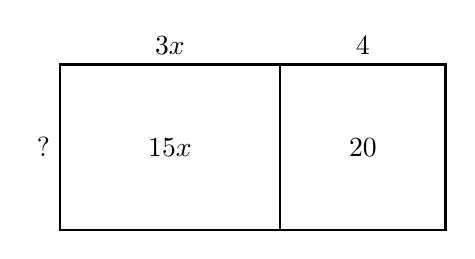
\begin{tikzpicture}[scale=0.7]
  \draw[thick] (0,0) rectangle (7,3);
  \draw[thick] (4,0) -- (4,3);
  \node[left] at (0,1.5) {?};
  \node[above] at (2,3) {$3x$};
  \node[above] at (5.5,3) {$4$};
  \node at (2,1.5) {$15x$};
  \node at (5.5,1.5) {$20$};
\end{tikzpicture}
\end{center}
\end{questionText}
\choiceA{$5(3x + 4)$}
\choiceB{$3(5x + 4)$}
\choiceC{$4(3x + 5)$}
\choiceD{$15(x + 20)$}
\correctAnswer{A}
\explanation{The width must satisfy: $? \times 3x = 15x$ and $? \times 4 = 20$. So $? = 5$. The factored form is $5(3x + 4) = 15x + 20$.}
\end{practiceQuestion}

\begin{practiceQuestion}{4-4-q27}{gmc}
\begin{questionText}
The arrays below show how $12$ tiles can be arranged. Which arrangement shows that $12 = 4 \times 3$?

\begin{center}
\begin{tikzpicture}[scale=0.5]
  % Arrangement A: 2 x 6
  \node[font=\bfseries] at (3, 3.5) {A: $2 \times 6$};
  \foreach \x in {0,...,5} {
    \foreach \y in {0,...,1} {
      \fill[funBlue!40] (\x+0.1, \y+0.1) rectangle (\x+0.9, \y+0.9);
      \draw[thick] (\x+0.1, \y+0.1) rectangle (\x+0.9, \y+0.9);
    }
  }
  % Arrangement B: 4 x 3
  \begin{scope}[xshift=8cm]
  \node[font=\bfseries] at (1.5, 5) {B: $4 \times 3$};
  \foreach \x in {0,...,2} {
    \foreach \y in {0,...,3} {
      \fill[funGreen!40] (\x+0.1, \y+0.1) rectangle (\x+0.9, \y+0.9);
      \draw[thick] (\x+0.1, \y+0.1) rectangle (\x+0.9, \y+0.9);
    }
  }
  \end{scope}
  % Arrangement C: 1 x 12
  \begin{scope}[xshift=13cm]
  \node[font=\bfseries] at (6, 1.5) {C: $1 \times 12$};
  \foreach \x in {0,...,11} {
    \fill[funOrange!40] (\x+0.1, 0.1) rectangle (\x+0.9, 0.9);
    \draw[thick] (\x+0.1, 0.1) rectangle (\x+0.9, 0.9);
  }
  \end{scope}
\end{tikzpicture}
\end{center}
\end{questionText}
\choiceA{Arrangement A}
\choiceB{Arrangement B}
\choiceC{Arrangement C}
\choiceD{All three arrangements}
\correctAnswer{B}
\explanation{Arrangement B shows $4$ rows and $3$ columns, illustrating $12 = 4 \times 3$. This connects to factoring: $12$ can be written as the product $4(3)$.}
\end{practiceQuestion}

\begin{practiceQuestion}{4-4-q28}{gmc}
\begin{questionText}
The rectangle below has the given area. Which pair of dimensions is correct?

\begin{center}
\begin{tikzpicture}[scale=0.7]
  \draw[thick, fill=funBlue!10] (0,0) rectangle (6,2.5);
  \node at (3,1.25) {Area $= 10x + 35$};
  \node[left] at (0,1.25) {?};
  \node[below] at (3,0) {?};
\end{tikzpicture}
\end{center}
\end{questionText}
\choiceA{Width $= 5$, Length $= 2x + 7$}
\choiceB{Width $= 10$, Length $= x + 35$}
\choiceC{Width $= 5$, Length $= 2x + 35$}
\choiceD{Width $= 2$, Length $= 5x + 35$}
\correctAnswer{A}
\explanation{Factor: $10x + 35 = 5(2x + 7)$. So the width is $5$ and the length is $2x + 7$.}
\end{practiceQuestion}

\begin{practiceQuestion}{4-4-q29}{gsa}
\begin{questionText}
The total area of the two rectangles shown below is $8x + 12$. Both rectangles have the same height $h$. Find the value of $h$.

\begin{center}
\begin{tikzpicture}[scale=0.7]
  \draw[thick, fill=funBlue!15] (0,0) rectangle (4,2.5);
  \node[below] at (2,0) {$2x$};
  \node[left] at (0,1.25) {$h$};
  \node at (2,1.25) {};
  \draw[thick, fill=funGreen!15] (5,0) rectangle (8,2.5);
  \node[below] at (6.5,0) {$3$};
  \node[right] at (8,1.25) {$h$};
\end{tikzpicture}
\end{center}
\end{questionText}
\correctAnswer{$h = 4$}
\explanation{Total area $= h(2x) + h(3) = h(2x + 3) = 8x + 12$. Factor: $8x + 12 = 4(2x + 3)$. So $h = 4$.}
\end{practiceQuestion}

\begin{practiceQuestion}{4-4-q30}{gsa}
\begin{questionText}
A store sells gift boxes. The cost for $n$ gift boxes and $n$ greeting cards is shown below. Factor the total cost completely.

\begin{center}
\begin{tabular}{|c|c|c|}
\hline
\textbf{Item} & \textbf{Price Each} & \textbf{Quantity} \\
\hline
Gift box & $\$6$ & $n$ \\
\hline
Greeting card & $\$3$ & $n$ \\
\hline
\multicolumn{2}{|c|}{\textbf{Total Cost}} & $6n + 3n$ \\
\hline
\end{tabular}
\end{center}
\end{questionText}
\correctAnswer{$3n(2 + 1) = 3n(3) = 9n$, or factored as $3n(2 + 1)$}
\explanation{Total cost $= 6n + 3n$. The GCF is $3n$. Factor: $6n \div 3n = 2$ and $3n \div 3n = 1$. So $6n + 3n = 3n(2 + 1) = 3n \times 3 = 9n$.}
\end{practiceQuestion}
